%----------------------------------------------------------------------------------------
%	PACKAGES AND THEMES
%----------------------------------------------------------------------------------------
\documentclass[aspectratio=169,xcolor=dvipsnames]{beamer}
\usetheme{Simple}

\usepackage{hyperref}
\usepackage{color}
\usepackage{listings}
\usepackage{ragged2e}
\usepackage{minted}
\usepackage [english,russian]{babel}
\usepackage{graphicx} % Allows including images
\usepackage{booktabs} % Allows the use of \toprule, \midrule and \bottomrule in tables



%----------------------------------------------------------------------------------------
%	TITLE PAGE
%----------------------------------------------------------------------------------------

% The title
\title[short title]{Разработка приложения \\ <<Курсы Валют>> }
\subtitle{Отчет о проектной работе по курсу <<Основы информатики и программирования>>}
\author[belenkov] {Николай Беленков}
\institute[NTU] % Your institution may be shorthand to save space
{
    % Your institution for the title page
    Институт Математики и Информационных Технологий \\
    Петрозаводский Государственный Университет
    \vskip 3pt
}
\date{17 января 2022} % Date, can be changed to a custom date


%----------------------------------------------------------------------------------------
%	PRESENTATION SLIDES
%----------------------------------------------------------------------------------------

\begin{document}

\lstdefinestyle{customc}{
  belowcaptionskip=1\baselineskip,
  breaklines=true,
  frame=L,
  xleftmargin=\parindent,
  language=C,
  showstringspaces=false,
  basicstyle=\footnotesize\ttfamily,
  keywordstyle=\bfseries\color{blue},
  commentstyle=\itshape\color{purple},
  identifierstyle=\color{black},
  stringstyle=\color{orange},
}
\lstdefinestyle{customasm}{
  belowcaptionskip=1\baselineskip,
  frame=L,
  xleftmargin=\parindent,
  language=[x86masm]Assembler,
  basicstyle=\footnotesize\ttfamily,
  commentstyle=\itshape\color{purple},
}

\lstset{escapechar=@,style=customc}

\begin{frame}
    % Print the title page as the first slide
    \titlepage
    \end{frame}

\begin{frame}{Содержание}
    \tableofcontents
\end{frame}

\section{Введение}

\begin{frame}[fragile]{Введение}
\begin{justifying}
Мобильные игры являются наиболее крупным и перспективным рынком в мире гейминга. При разработке мобильных игр применяются специальные игровые движки, а также языки, используемые для разработки мобильных приложения - Java и Kotlin, последний язык появился не так давно(в 2011 году) и представляет для автора наибольший интерес среди представленных средств разработки.

Для того, чтобы получить опыт в мобильной разработке я решил реализовать на Kotlin несложную карточную игру <<Мавр>>. Таким образом, целью данного проекта стала разработка приложения, позволяющего проводить время за игрой в <<Мавр>>, ставший популярным в России еще в 19 веке. Данная карточная игра является весьма интересной и не забытой до сих пор.
\end{justifying}
\end{frame}

\section{Цели и задачи проекта}
\begin{frame}[fragile]{Цели и задачи проекта}
Цель проекта: Разработать мобильное приложение, дающее возможность играть в <<Мавр>> (также известа как <<101>>, <<Чешский дурак>> и т.д.).
\newline\newline
Задачи проекта: 
%%% Пример создания списков %%%
\begin{enumerate} 
    \item Разработать прототип приложения с применением C++.
    \item Спроектировать интерфейс приложения.
    \item Перенести логику приложения на Kotlin.
    \item Реализовать интерфейс приложения на Kotlin.
    \item Проверить возжность использования приложения для игры.
\end{enumerate}
\end{frame}

\section{Прототип}
\begin{frame}{Прототип приложения}
В начале разработки было решено реализовать логику приложения на C++ с применением текстового интерфейса/
    \begin{figure}
        \centering
        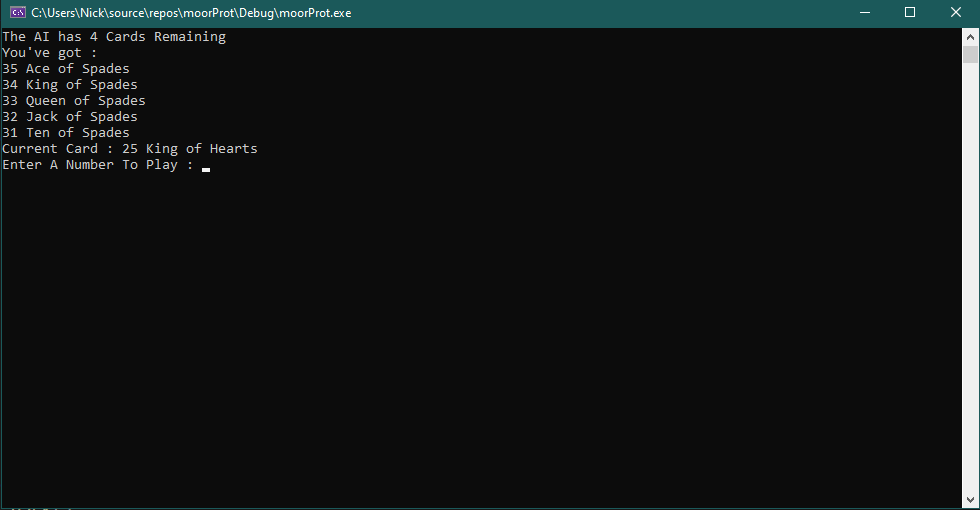
\includegraphics[scale=0.4]{prototype.png}
        \caption{Прототип игры на C++}
        \label{fig:my_label}
    \end{figure}
    
\end{frame}
\section{Приложение на Kotlin}
\begin{frame}[fragile]{Пример функции на Kotlin}
\begin{minted}{text}
    private fun addCardtoAI(number: Int) {
        val imageButton = ImageButton(this)
        imageButton.layoutParams = LinearLayout.LayoutParams(
            250,
            ViewGroup.LayoutParams.MATCH_PARENT
        )
        imageButton.scaleType = ImageView.ScaleType.CENTER_CROP;
        imageButton.id= number
        imageButton.setImageResource(cardsArray[number])
        imageButton.setOnClickListener {
            tryToPlay(1,number)
        }
        // Add ImageButton to LinearLayout
        hLayout2.addView(imageButton)
    }
\end{minted}
    
\end{frame}
\begin{frame}{Интерфейс приложения}
    \begin{figure}
        \centering
        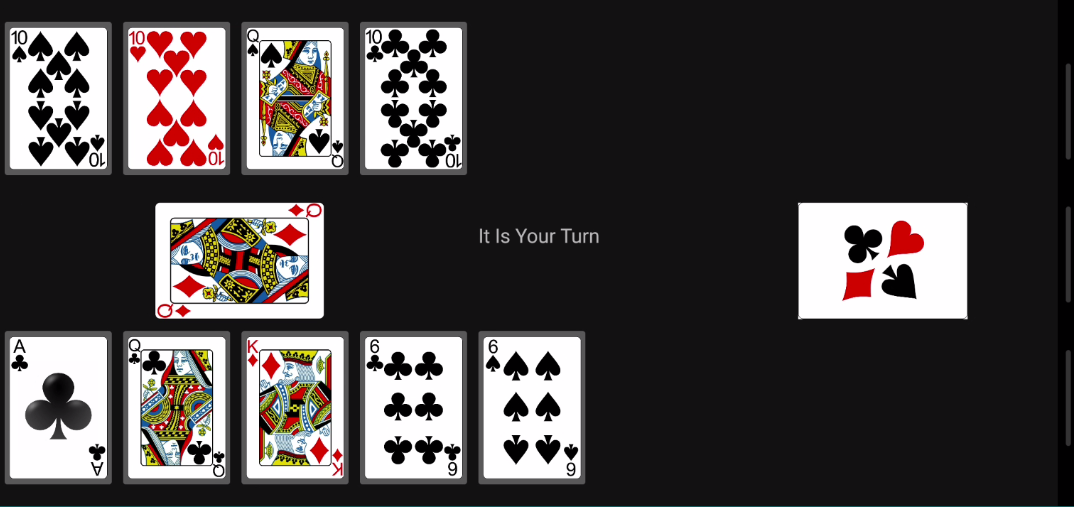
\includegraphics[scale=0.4]{interface.png}
        \caption{Интерфейс разработанного приложения}
        \label{fig:my_label}
    \end{figure}
\end{frame}

\section{Заключение}
\begin{frame}{Заключение}
\begin{justifying}
В результате нам удалось разработать приложение, которое позволяет играть в <<Мавр>>, также известный как <<101>>, игра следует основным правилам, описанным в приложении А, и имеет удобный интерфейс, адаптирующийся под различное количество карт на руке игрока. Итоговое приложение реализовано полностью с помощью Android Studio и языка Kotlin. 

Были использованы различные возможности Android Studio для реализации интерфейса : TextView, ImageView, ImageButton. ScrollView, различные варианты Layout.

\parВ ходе данной работы я получил опыт работы функциями языка Kotlin - основы программирования с помощью языка, в т.ч. ветвления, циклы, контейнеры и т.д., а также с возможностями Android Studio по созданию интерфейса мобильного приложения.
\end{justifying}
\end{frame}

%----------------------------------------------------------------------------------------

\end{document}